\documentclass{scrartcl}
\usepackage[ngerman]{babel}
\usepackage{fontspec,microtype,hyperref,tikz,booktabs,float,graphicx}%\usepackage{lua-visual-debug}
\usetikzlibrary{positioning,shapes.geometric,shapes.multipart}
\hypersetup{colorlinks=false,pdfborder={0 0 0}}
\tikzset{
	>=latex,
}

\title{COSMIC}
\subtitle{Protokoll zum Projekt im Modul „Molekularbiologische Datenbanken“}
\author{%
	Thomas Dencker\thanks{\url{mailto:thomas.dencker@stud.uni-goettingen.de}} \and
	Robert Kratel\thanks{\url{mailto:robert.kratel@stud.uni-goettingen.de}} \and
	Pascal Schmitt\thanks{\url{mailto:pascal.schmitt1@stud.uni-goettingen.de}}}
\begin{document}
\maketitle
\vfill
\tableofcontents
\newpage

\section{Aufgabenstellung}

Die Aufgabenstellung des Datenbankprojektes war es, eine auf SQLite\footnote{\url{http://sqlite.org/}} basierende Datenbank aufzubauen. Den Ausgangspunkt dieser Datenbank stellt eine Liste von „UniProt accession numbers“ dar. Die Datenbank sollte Informationen aus den entsprechenden Einträgen der UniProt\footnote{\url{http://uniprot.org/}}-Datenbank enthalten, wie den Protein- und Gennamen. Den Gennamen sollten außerdem alle Synonyme zugeordnet werden, welche in der GeneNames\footnote{\url{http://genenames.org/}}-Datenbank gespeichert sind. Neben diesen allgemeinen Aufgaben sollten kodierende und nichtkodierende Mutationen in Krebserkranken in den Genen der Datenbank identifiziert werden. Diese Informationen sollten der COSMIC\footnote{\url{http://cancer.sanger.ac.uk/cancergenome/projects/studies/}}-Datenbank entnommen werden. Darüber hinaus sollte das relationale Datenbank-Schema auf Grundlage eines Entity-Relationship-Modells entworfen werden.

Das Projekt kombiniert Informationen aus drei Datenbanken, deren Inhalt im Folgenden kurz beschrieben wird.

\begin{description}
\item[UniProt]
Die UniProt-Datenbank ist eine freizugängliche Datenbank, die Sequenzen und funktionelle Informationen zu Proteinen enthält. Diese werden von der Swiss-Prot- und der TrEMBL-Datenbank bereitgestellt. Die Einträge der Datenbank können u.a. durch die UniProtJAPI abgefragt und gespeichert werden.
\item[GeneNames]
genenames.org ist eine Datenbank, welche vom HGNC(HUGO Gene Nomenclature Committee) akzeptierte Gennomenklatur enthält. Unter anderem sind das anerkannte Symbol, die vorherigen Symbole und Synonyme zu rund 19000 proteinkodierenden Genen downloadbar.
\item[COSMIC]
Die COSMIC-Datenbank wird vom Sanger-Institut bereitgestellt und enthält Informationen zu somatischen kodierenden und nicht-kodierenden Mutationen in Krebserkrankungen.
\end{description}

\newpage
\section{Entity-Relationship-Modell}

\begin{figure}\centering
	\begin{tikzpicture}[x=5pt,y=20pt,
		entity/.style={rectangle, draw, inner sep=8pt, fill=black!10},
		rel/.style={diamond, aspect=2, draw, font=\small, inner sep=2pt, fill=white},
		attr/.style={rectangle, rounded corners=6pt, draw, font=\footnotesize, anchor=west},
		attl/.style={attr, anchor=east},
		primary/.style={font=\footnotesize\it},
		shorten >=1pt,
	]
		\draw
			node(gene)[entity]{Gen}
				(gene.south) -- ++(0,-1) coordinate(k) -- ++(-1,0) node[attl,primary]{Name}
				(k) -- ++(0,-1) coordinate(k) -- ++(-1,0) node[attl]{Alte Namen}
				(k) -- ++(0,-1) coordinate(k) -- ++(-1,0) node[attl]{Alternative Namen}
				(k) -- ++(0,-1) coordinate(k) -- ++(-1,0) node[attl,dashed]{Sequenz}
			node(mut)[entity,above=60pt of gene]{Mutation}
				(mut.west) -- ++(-1,0) coordinate(k) -- ++(-1,0) node[attl,primary]{COSMIC-ID}
				(k) -- ++(0,-1) coordinate(k) -- ++(-1,0) node[attl]{Codierend?}
				(k) -- ++(0,-1) coordinate(k) -- ++(-1,0) node[attl]{Position}
				(k) -- ++(0,-1) coordinate(k) -- ++(-1,0) node[attl]{Referenz-Sequenz}
				(k) -- ++(0,-1) coordinate(k) -- ++(-1,0) node[attl]{Alternativ-Sequenz}
				(k) -- ++(0,-1) coordinate(k) -- ++(-1,0) node[attl]{AS-Differenz}
			node(prot)[entity,right=120pt of gene]{Protein}
				(prot.south) -- ++(0,-1) coordinate(k) -- ++(1,0) node[attr]{Name}
				(k) -- ++(0,-1) coordinate(k) -- ++(1,0) node[attr,primary]{Uniprot-ID}
				(k) -- ++(0,-1) coordinate(k) -- ++(1,0) node[attr]{Accession-Nr.}
				(k) -- ++(0,-1) coordinate(k) -- ++(1,0) node[attr]{Sequenz}
			node(iso)[entity,above=60pt of prot]{Isoform}
				(iso.east) -- ++(1,0) coordinate(k) -- ++(1,0) node[attr,primary]{Name}
				(k) -- ++(0,-1) coordinate(k) -- ++(1,0) node[attr]{alt. Sequenz}
		;
		\draw[->] (mut) -- (gene) node[pos=0.15,right]{$n$} node[pos=0.5,rel]{von} node[pos=0.85,right]{$1$};
		\draw[->] (iso) -- (prot) node[pos=0.15,right]{$n$} node[pos=0.5,rel]{von} node[pos=0.85,right]{$1$};
		\draw[->] (gene) -- (prot) node[pos=0.1,above]{$n$} node[pos=0.5,rel]{erzeugt} node[pos=0.9,above]{$n$};
		\draw[->,dashed] (mut) -- (iso) node[pos=0.1,above]{$n$} node[pos=0.9,above]{$1$};
	\end{tikzpicture}
	\caption{Entity-Relationship-Modell}\label{ermodel}
\end{figure}

Ausgangspunkt der Datenbank sind die durch die „UniProt accession numbers“ referenzierten Proteine. Als Attribute wurden der in der Aufgabenstellung geforderte Proteinname, die UniProtID und die Accession Number gewählt, über die weitere Informationen abgerufen werden könnten. Außerdem gibt es die Aminosäuresequenz als weiteres Attribut, um diese ggf. mit den Sequenzen der Isoformen vergleichen zu können.

Proteine sind Produkte eines oder mehrerer Gene ($n:n$), da hier keine Gendatenbank verwendet wird, speichern wir die Basensequenz der Gene und ihre Position im Genom nicht. Die Genenames-Datenbank enthält Informationen über den offiziellen, alternative und alte Namen für Gene, wobei COSMIC und UniProt nicht durchgehend den aktuellen offiziellen Namen verwenden. Gene können mehrere Mutationen besitzen ($1:n$), wobei die COSMIC-Datenbank speichert welche Basenpaare der Referenz-Sequenz eines Gens durch alternative Basenpaare ersetzt werden und ob dies Auswirkungen auf das erzeugte Protein hat. Falls ja wird diese Mutation „kodierend“ genannt und COSMIC speichert zusätzlich die resultierende Änderung an der Aminosäuresequenz des Proteins, was eine Isoform des Proteins erzeugt ($1:n$). UniProt und COSMIC speichern allerdings nicht, welche Mutation zu welcher Isoform gehört ($n:1$), daher ist dies nicht Teil unseres Modells.

\newpage
\section{Implementierung}

Das im Rahmen dieses Projekts erstellte Programm liest Daten aus den Quelldatenbanken ein, speichert sie in einer eigenen SQLite-basierten Datenbank und führt darauf Abfragen aus.

Zum Einlesen und Speichern der Daten wurde als Programmiersprache Java gewählt, da es für die UniProt-Datenbank eine Java-Schnittstelle gibt und die Daten einfach über JDBC in die SQLlite-Datenbank eingespeichert werden können. Zum Ausführen der Abfragen wurde eine einfache GUI erstellt, die eine SQL-Anfrage entgegennimmt und nach Ausführen das Ergebnis bzw. die Fehlermeldung darstellt.

\subsection{Relationales Datenbank-Schema}

\begin{figure}\centering
	\begin{tikzpicture}[
		table/.style={
			rectangle split, rectangle split parts=#1,
			rectangle split draw splits=false,
			rectangle split part fill={black!10,white},
			rectangle split part align={left},
			draw, font=\tt,
		},
		shorten >=1pt,
	]
	\def\p#1{\nodepart{#1}\vphantom{qd}}
		\draw
			node(mut)[table=7]{%
				\vphantom{q}mutation
				\p{two}\itshape id
				\p{three}gene
				\p{four}coding
				\p{five}position
				\p{six}reference
				\p{seven}...}
			node(syn)[table=4,right=of mut.three east,anchor=three west]{%
				\vphantom{d}synonym
				\p{two}\itshape official
				\p{three}\itshape name
				\p{four}kind}
			%node(synv)[table=4,below=of syn,dashed]{%
			%	\vphantom{d}genename
			%	\p{two}official
			%	\p{three}\itshape a
			%	\p{four}\itshape b}
			node(prod)[table=3,right=of syn.three east,anchor=two west]{%
				\vphantom{d}product
				\p{two}\itshape gene
				\p{three}\itshape protein}
			node(prot)[table=5,right=of prod.three east,anchor=two west]{%
				protein
				\p{two}\itshape id
				\p{three}name
				\p{four}accession
				\p{five}sequence}
			node(iso)[table=4,right=of prot.two east,anchor=three west]{%
				\vphantom{q}isoform
				\p{two}\itshape id
				\p{three}protein
				\p{four}sequence}
		;
		\draw[->] (mut.three east) to (syn.three west);
		\draw[->] (syn.three east) to (prod.two west);
		\draw[->] (prod.three east) to (prot.two west);
		\draw[->] (iso.three west) to (prot.two east);
		%\draw[->,shorten <=3pt,out=-45,in=180] (mut.three east) to (synv.three west);
		%\draw[->,shorten >=5pt,out=0,in=180+45] (synv.four east) to (prod.two west);
	\end{tikzpicture}
	\caption{Datenbanktabellen und Referenzen}\label{tables}
\end{figure}

Das Entity-Relationship-Modell aus Abb.~\ref{ermodel} wurde in ein relationales Datenbankschema (siehe Abb.~\ref{tables}) überführt, dabei ist zu beachten dass hier keine explizite \texttt{gene}-Tabelle existiert sondern die beiden $n:n$ und $n:n$-Relationen \texttt{synonym} und \texttt{product} direkt gejoined werden. Dabei ist zu beachten dass \texttt{mutation.gene} und \texttt{product.gene} keine Foreign Keys auf \texttt{synonym.name} sind, da beide verschiedene Alternativen zum offiziellen Namen verwenden könnten.
\begin{verbatim}
CREATE TABLE synonym (official, name, kind,
                      PRIMARY KEY (official, name));
CREATE TABLE mutation (id PRIMARY KEY, gene, coding, position,
                       reference, alternative, strand, aa, count);
\end{verbatim}
Die UniProt-Referenzen auf Protein-IDs sind allerdings eindeutig und wurden als Foreign Keys definiert. Im Gegensatz zu anderen Datenbanken unterstützt SQLite keine Datentyp-Annotationen für Spalten und speichert alles als Zeichenketten.
\begin{verbatim}
CREATE TABLE protein (id PRIMARY KEY, name, accession, sequence);
CREATE TABLE product (gene, protein REFERENCES protein(id),
                      PRIMARY KEY(gene, protein));
CREATE TABLE isoform (id PRIMARY KEY, protein REFERENCES protein(id),
                      sequence);
\end{verbatim}
Die Synonymtabelle speichert den offiziellen und alternative Namen. Allerdings verwenden weder UniProt noch COSMIC für sämtliche Gene die offiziellen Namen, Joins müssen daher symmetrisch erfolgen. Der Einfachheit halber wird diese symmetrische Relation als View definiert.
\begin{verbatim}
CREATE VIEW genename AS
SELECT DISTINCT s1.name AS a, s2.name AS b, s2.official
FROM synonym s1, synonym s2 WHERE s1.official = s2.official;
\end{verbatim}
Um Abfragen weiter zuvereinfachen, wird der Join von Mutationen über Synonyme und Genprodukten zu Proteinen in eine weitere View zusammengefasst. Um in Abfragen weitere Joins zu vermeiden und die Abfragen zu beschleunigen wird eine temporäre Tabelle als Zwischenspeicher verwendet.
\begin{verbatim}
CREATE TEMP TABLE proteinmut AS
SELECT m.id AS mid, m.*, p.id AS pid, p.*, n.official AS gene
FROM mutation m, genename n, product g, protein p
WHERE m.gene = n.a AND n.b = g.gene AND g.protein = p.id;
\end{verbatim}

\subsection{Einlesen der Daten}

\begin{description}
\item[UniProt]
Bevor die UniProt-Einträge abgefragt werden konnten, musste zunächst die \texttt{uniprot.acc}-Datei geparst werden. Dabei musste berücksichtigt werden, dass die Liste Duplikate enthielt. Diese wurden aussortiert, um unnötige Anfragen an die UniProt-Datenbank zu sparen.

Darüber hinaus musste die Liste geteilt werden, da der durch die UniProtJAPI vorgestellte \texttt{UniProtQueryBuilder} nur Listen mit maximal 1024 Einträgen unterstützt. Sind die entsprechenden Daten nicht bereits in der Datenbank enthalten, werden die UniProt-Einträge von der Datenbank abgefragt und der empfohlene Name in der Proteinbeschreibung, die UniProtID, die primäre „accession number“, die Gennamen und die Isoformen (beschrieben durch „Alternative Products“ in den Kommentaren) durch entsprechende Funktionen der UniProtJAPI ausgelesen.
Einige Eintäge, z.B. \texttt{Q8WUN3}, \texttt{Q6N045} und \texttt{A6NF79} existieren nicht mehr und wurden daher ignoriert.

\item[GeneNames]
Auf der GeneNames-Website kann der Datenbestand in diversen Formaten abgefragt werden, unser Programm lädt die Daten in einem Tab-separierten Format per HTTP herunter, parst sie zeilenweise und schreibt sie in die \texttt{synonym}-Tabelle. Die Spalte „Approved Symbol“ enthält dabei den offiziellen Namen, in „Previous Symbols“ und „Synonyms“ stehen, durch Komma getrennt, alternative Namen. Für jede Kombination dieser Namen mit dem offiziellen Namen wird eine Zeile eingefügt und in der \texttt{kind}-Spalte entsprechend \texttt{previous} oder \texttt{alias} vermerkt. Der offizielle Name verweist auch auf sich selbst, dies wird mit \texttt{refl} markiert.

Dieser Ansatz ist allerdings mehrdeutig: so führt GeneNames z.B. \texttt{ARX} als neuen offiziellen Namen für \texttt{PRTS} auf, und auch \texttt{ARX} als Synonym zu \texttt{UBA2}, aber nicht umgekehrt. Auf solche Inkonsistenzen wird keine Rücksicht genommen und die Daten so verwendet, als gäbe es einen offiziellen Namen für jedes Gen, in dessen Zeile im GeneNames-Datensatz alle Synonyme aufgeführt werden.

\item[COSMIC]
Die Listen der kodierenden und nichtkodierenden Genmutationen werden, sofern sie veraltet sind, vom FTP-Server des Sanger-Instituts geladen. Sie liegen mittels GZip gepackt im „Variant Call Format“ (VCF) vor, ein auf dem Tab-separierten Format basierendes Textformat das für die Speicherung von SNPs entworfen wurde. Für jede Mutation ist das Chromosom, die Position, Ursprungs- und Alternativsequenz angegeben. Falls die Mutation in einem Gen liegt, wird in der Info-Spalte auch der Genname genannt, dies ist bei allen kodierenden Mutationen der Fall. Einige nichtkodierende Mutationen liegen ebenfalls innerhalb eines Gens, allerdings z.B. in Introns, wirken sich also nicht auf das Endprodukt aus. Alles wird in die \texttt{mutation}-Tabelle geschrieben.
\end{description}

\section{Abfragen}

Mit der einfachen GUI können SQL-Anfragen ausgeführt werden um komplizierte Fragen zu beantworten wie in Tabellen~\ref{q1}, \ref{q2}, \ref{q3}, \ref{q4}, \ref{q5} und \ref{q6} aufgeführt.

\begin{table}[H]
	\noindent\begin{minipage}{.4\hsize}
	\begin{verbatim}
	SELECT p.name,
	       GROUP_CONCAT(g.gene)
	FROM protein p, product g
	WHERE g.protein = p.id
	GROUP BY p.id
	HAVING COUNT(*) > 1
	\end{verbatim}
	\end{minipage}
	\begin{minipage}{.6\hsize}
	\hfill\begin{tabular}{ll}
	\toprule
	Protein & Gene\\
	\midrule
	Basic helix-loop-helix T.F.&\texttt{DMRTC1,DMRTC1B}\\
	Doublesex-\& mab-3-rel. T.F.&\texttt{HSDX1,HSFX2}\\
	Heat shock T.F., X-linked&\texttt{HSFY1,HSFY2}\\
	Heat shock T.F., Y-linked&\texttt{SCXA,SCXB}\\
	\bottomrule
	\end{tabular}
	\end{minipage}
	\caption{Welche Proteine werden von mehr als einem Gen kodiert?}\label{q1}
\end{table}

\begin{table}[H]
	\noindent\begin{minipage}{.5\hsize}
	\begin{verbatim}
	SELECT gene, mid, aa
	FROM proteinmut
	WHERE pid = "DMRTC_HUMAN"
	\end{verbatim}
	\end{minipage}
	\begin{minipage}{.5\hsize}
	\hfill\begin{tabular}{lll}
	\toprule
	Gen&COSMIC-ID&Prot.-Mutation\\
	\midrule
	\texttt{DMRTC1}&\texttt{COSM458031}&\texttt{p.R171G} \\
	\texttt{DMRTC1}&\texttt{COSM195610}&\texttt{p.G159V} \\
	\bottomrule
	\end{tabular}
	\end{minipage}
	\caption{Welche Mutationen beeinflussen das DMRTC-Protein?}\label{q2}
\end{table}

\begin{table}[H]
	\noindent\begin{minipage}{.65\hsize}
	\begin{verbatim}
	SELECT DISTINCT gene, accession
	FROM proteinmut
	WHERE CAST(position AS INTEGER) > 1700000
	AND   CAST(position AS INTEGER) < 2000000
	ORDER BY position
	\end{verbatim}
	\end{minipage}
	\begin{minipage}{.35\hsize}
	\hfill\begin{tabular}{ll}
	\toprule
	Gen & Acc\# \\
	\midrule
	\texttt{CRAMP1L}&\texttt{Q96RY5}\\
	\texttt{ONECUT3}&\texttt{O60422}\\
	\texttt{MYT1L}&\texttt{Q9UL68}\\
	\texttt{KLF16}&\texttt{Q9BXK1}\\
	\texttt{IRX4}&\texttt{P78413}\\
	\texttt{WHSC1}&\texttt{O96028}\\
	\texttt{HIC1}&\texttt{Q14526}\\
	\bottomrule
	\end{tabular}
	\end{minipage}
	\caption{Welche Proteine stammen aus einem best. Abschnitt des Genoms?}\label{q3}
\end{table}

\begin{table}[H]
	\noindent\begin{minipage}{.4\hsize}
	\begin{verbatim}
	SELECT m.name,
	       i.iso AS isoforms,
	       COUNT(*) AS mutations,
	       SUM(m.count) AS cases
	FROM proteinmut m,
	     (SELECT protein,
	             COUNT(*) AS iso
	      FROM isoform
	      GROUP BY protein
	      HAVING iso >= 10
	      ORDER BY iso DESC) i
	WHERE i.protein = m.pid
	GROUP BY m.pid
	ORDER BY cases DESC
	\end{verbatim}
	\end{minipage}
	\begin{minipage}{.6\hsize}
	\hfill\begin{tabular}{lrrr}
	\toprule
	Name & \#Iso & Stellen & Fälle \\
	\midrule
	Runt-related TF 1&11&223&303\\
	TF 4&11&196&152\\
	TF 7-like 2&12&122&103\\
	Homeobox prot...&11&112&95\\
	Tumor protein 63&12&81&74\\
	Zinc finger prot...&15&58&51\\
	Glucocorticoid receptor&10&43&41\\
	NF of act. T-cells...&24&38&40\\
	Microphthalmia-ass. TF&11&39&36\\
	Tumor prot. p73&10&23&24\\
	Nuclear receptor...&11&19&16\\
	cAMP-resp. el...&23&21&15\\
	TF 7&16&16&12\\
	\bottomrule
	\end{tabular}
	\end{minipage}
	\caption{Wie viele Genmutationen wirken auf die Proteine mit den meisten Isoformen?}\label{q4}
\end{table}

\begin{table}[H]
	\noindent\begin{minipage}{.4\hsize}
	\begin{verbatim}
	SELECT reference, alternative, COUNT(*)
	FROM mutation
	GROUP BY reference, alternative
	ORDER BY COUNT(*) DESC
	LIMIT 5
	\end{verbatim}
	\end{minipage}
	\begin{minipage}{.6\hsize}
	\hfill\begin{tabular}{ccr}
	\toprule
	von & nach & Fälle \\
	\midrule
	C&T&142508\\
	G&A&141469\\
	C&A&105685\\
	G&T&104645\\
	T&C&40654\\
	\bottomrule
	\end{tabular}
	\end{minipage}
	\caption{Welche Mutationen sind am häufigsten?}\label{q5}
\end{table}

\begin{table}[H]
	\noindent\begin{minipage}{.4\hsize}
	\begin{verbatim}
	SELECT
	  CASE LENGTH(reference) > LENGTH(alternative) WHEN 1
	    THEN "Deletion"
	    ELSE CASE LENGTH(reference) = LENGTH(alternative) WHEN 1
	      THEN "Mutation"
	      ELSE "Insertion"
	    END
	  END AS kind, COUNT(*)
	FROM mutation
	GROUP BY kind ORDER BY COUNT(*) DESC
	\end{verbatim}
	\end{minipage}
	\begin{minipage}{.6\hsize}\vspace{2cm}
	\hfill\begin{tabular}{lr}
	\toprule
	Art & Fälle \\
	\midrule
	Mutation&734690 \\
	Deletion&15964 \\
	Insertion&7261 \\
	\bottomrule
	\end{tabular}
	\end{minipage}
	\caption{Welche Arten von Änderungen sind am häufigsten?}\label{q6}
\end{table}

\begin{table}[H]
	\noindent\begin{minipage}{.5\hsize}
	\begin{verbatim}
	SELECT DISTINCT
	     m.gene,     n.official, g.gene
	FROM mutation m, genename n, product g
	WHERE m.gene = n.a AND n.b = g.gene
	AND m.gene != g.gene
	LIMIT 4
	\end{verbatim}
	\end{minipage}
	\begin{minipage}{.5\hsize}
	\hfill\begin{tabular}{ccc}
	\toprule
	COSMIC & GeneNames & UniProt \\
	\midrule
	\texttt{MGC33414}&\texttt{ZNF683}&\texttt{ZNF683}\\
	\texttt{CREB3L4}&\texttt{CREB3L4}&\texttt{CREB3}\\
	\texttt{TCF7L2}&\texttt{TCF7L2}&\texttt{TCF4}\\
	\texttt{RNF141}&\texttt{RNF141}&\texttt{ZNF230}\\
	\bottomrule
	\end{tabular}
	\end{minipage}
	\caption{Beide Datenbanken folgen nicht immer der offiziellen Benennung}\label{q7}
\end{table}

\begin{figure}[H]\centering
	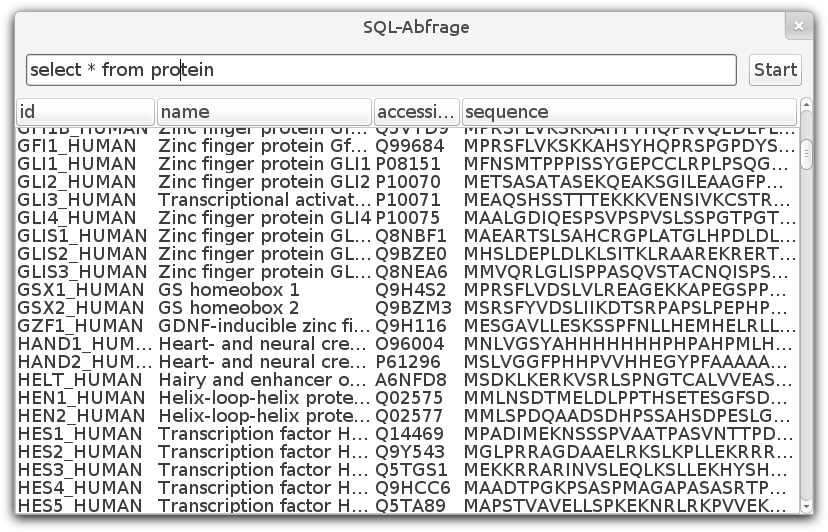
\includegraphics[height=8cm]{screenshot}
	\caption{Bildschirmfoto der GUI}
\end{figure}

\end{document}
